\section{Exercise 5: Drupal}
\subsection{Background}
\subsubsection{Which vulnerabilities do you think can be used? Pick two potential vulnerabilities and describe them in terms of why you picked them, i.e., date and exploit effect.}
The vulnerabilities that I'd pick are the drupal\_coder\_exec vulnerability and the drupal\_drupageddon vulnerability. Both of these have an excellent rank in terms of exploitability.
\\\\
The drupal\_coder\_exec exploit is a good choice because of the fact that a third-party plugin is introducing the vulnerability. This means that drupal, as an organization don't have as much control over the issue as they otherwise would if the exploit came from in-house code. The fact that the module allows for arbitrary code execution also means, that it's potentially a powerful entry point for a bad actor to use to gain access to further systems on the drupal server.
\\\\
The drupal\_drupageddon exploit is a good choice, as it is a SQL injection exploit. Drupal being a CMS makes this especially volatile, as usually, content pages for users using a CMS will be stored in some database, which the CMS then renders, effectively making entire websites available to bad actors gaining access using SQL injection. This is also the reason why the exploit was dubbed drupageddon, as it caused mass amounts of issues.
\subsubsection{For the rest of the tutorial, we will use the vulnerability \textit{dubbed drupageddon.} What is the underlying vulnerability?}
As explained before, the underlying vulnerability is an SQL injection vulnerability.

\subsubsection{What is so severe about the issue?}
As also explained before, all of the website content being stored in a database since Drupal is a CMS, it effectively allows a bad actor to access entire databases without authorization.

\subsection{Post-Exploitation}
\subsubsection{What are possible activities/aims for the post-exploitation phase?}
Now that we have access to the machine, our first goal is to establish persistence through a user account that we can sign in to the server with, gathering as much information about the target machine as possible, as well as possibly gaining higher privileges within the machine, so that we can gather even more information.

\subsubsection{Write out the list in the file that has the “User Accounts”?}
\lstinputlisting[caption={User List Output}]{Outputs/E05/msf\space -\space userlist.txt}

\subsubsection{How does having a list of user names help?}
Having a list of usernames help us by making brute force attacks easier to perform, as there is one less variable that we need to guess. It allows us to perform phishing campaigns, by using the information we have access to, to seem more credible. If the user has used the same username on multiple sites and perhaps even the same passwords, we can check known password databases for a password that we can try to use to enter the website.

\subsubsection{What do the excellent post exploitation scripts for linux offer?}
It offers us system information such as versions, directories, usernames, access to persistence through backdoors and more.

\subsection{Reflection}

\subsubsection{What is the main issue with the web server? How did it help selecting potential exploits?}
The web server has an exposed directory listing, which not only allows us to see the exact locaton of the drupal files, but also to access drupal through the drupal\_drupageddon exploit, gaining access to the host machine.

\subsubsection{When opening the drupal web page, you are greeted by a warning. Do you think this is good practice? Why or why not?}
The warnings are not good practice, as they disclose information about the application configuration that an attacker could use to gain further access to security vulnerabilities. It also gives away the fact, that the drupal server is misconfigured and might give way to further security vulnerabilities.

\subsubsection{Given a more restrictive web server configuration, finding the relevant information wouldn't have been that easy. Please check dirbuster, to be found in the “Web Application Analysis” menu. How could this tool help you finding information? Try it out on the Ubuntu metasploitable VM. Use /usr/share/dirbuster/wordlists/directory-list-2.3-medium.txt as dictionary.}
Dirbuster can help you find information about directories on a target server, by brute-forcing the directories, performing several requests to try and figure out what directories are present on the server and generating a report containing all that information. For example, if we wanted to use dirbuster to figure out what directories are in the /drupal directory, that we figured out earlier exists, we could use dirbuster as so

\begin{figure}[H]
  \caption{The Dirbuster User Interface}
  \begin{center}
    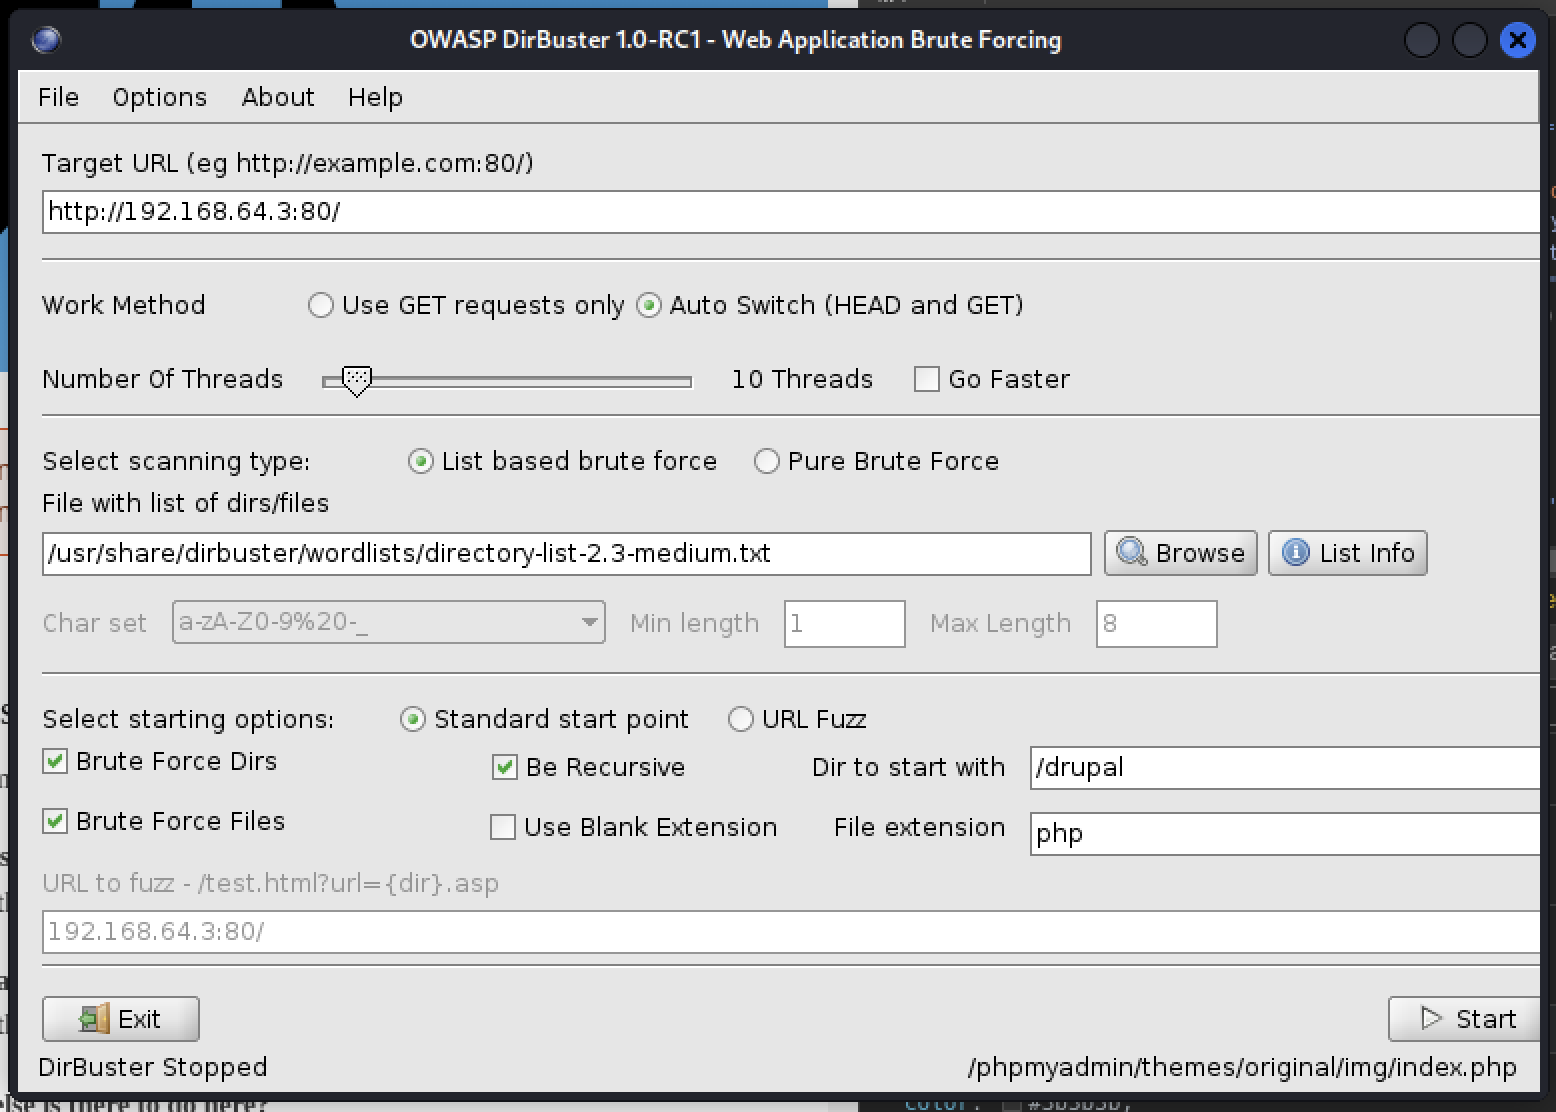
\includegraphics[width=\textwidth]{Outputs/E05/dirbuster.png}
  \end{center}
\end{figure}


\subsubsection{How can effective spying with tools like dirbuster prevented?}
There are several ways of which you can attempt to prevent tools like dirbuster being used:

\begin{itemize}
  \item Using custom directory names as opposed to default well-known ones.
  \item Implementing rate-limiting for single users, as dirbuster performs many requests.
  \item Implementing required CAPTCHAs when accessing the site.
  \item Implementing firewalls and setting up monitoring with alerts.
\end{itemize}

\subsubsection{This attack didn't get us all the way to root. How would you continue the pentest? What would be your next actions?}
While we didn't get all the way to the root user, gaining access to the root user is actually a rather simple feat now that we have access to a sudo user. We can simply use the passwd command as such: sudo passwd root, which will prompt us to give root a new password, which we can then use to login to root. These would be my next steps.

\subsubsection{Do you have any specific things in mind you would try to get root access?}
As stated before, I would attempt to use the passwd command to change the root password, which, could gain us access to the root user and gain full access of the system depending on the configuration. Considering the woefully misconfigured system, it's not so far-fetched that the system would be configured as such, that this was possible.

\subsubsection{What makes getting a remote shell so powerful?}
Getting a remote shell is especially powerful, as you now have access to running any commands that you desire. If you have root access, you can even move, copy and destroy any files you want. You could install new exploitative software, create backdoors and more. Having access to a remote shell means no longer being limited to simple injection attacks, but having much more control.